%TITULO------------------------------------------------------------------------

%==============================================================================
\chapter{Controle Multimalha Adaptativo}\label{controle}
%==============================================================================

	A modelagem desenvolvida separa a planta em duas partes: $G_{id}$ pertence à malha
    interna, e $G_{od}$ pertence à malha externa. Esta forma de modelagem permite isolar
    a incerteza paramétrica em $G_{od}$, de forma que o controlador projetado para a
    malha interna trata de uma planta com parâmetros conhecidos e projetados. Dessa forma,
    pode-se utilizar controladores convencionais para realizar o amortecimento ativo.

    É conhecido da literatura que, no caso específico de um filtro LCL, é suficiente
    para a realização do amortecimento da ressonância do filtro a utilização de um
    controlador proporcional, quando a variável intermediária escolhida é a corrente do
    capacitor, e de um controlador proporcional-derivativo, quando a variável intermediária
    escolhida é a tensão do capacitor~\cite{ref:DANNEHL}. O critério de escolha para a
    variável intermediária varia de acordo com a aplicação e a topologia~\cite{ref:POH}.

    Levando isto em consideração, neste trabalho um controlador proporcional é projetado
    para o caso da variável intermediária ser a corrente do capacitor, e um controlador
    proporcional-derivativo é projetado para o caso da variável intermediária ser a
    tensão do capacitor. O projeto de ambos leva em consideração os parâmetros listados
    na Tabela~\ref{tab:sim_parameters}.

    \begin{table}[htb]
        \renewcommand{\arraystretch}{1.35}
        \setlength{\tabcolsep}{1.2mm}
        \caption{Parâmetros do sistema utilizados no projeto.}
        \label{tab:sim_parameters}
        \centering
        \begin{tabular}{l l l l}
            \hline
            \multicolumn{1}{c}{Parâmetro} & \multicolumn{1}{c}{Valor} &
            \multicolumn{1}{c}{Parâmetro} & \multicolumn{1}{c}{Valor} \\
            \hline
            $L_1$ &  $2$mH      &  $L_2$                                   &  $2$mH    \\
            $C$   &  $40\mu$F   & Frequência de Amostragem ($f_s = 1/T_s$) &  $12$kHz  \\
            \hline
        \end{tabular}
    \end{table}


\section{Projeto para $U_p = V_C$}

    Considerando o controlador da malha interna $C_i(z)$ como sendo proporcional-derivativo,
    tem-se sua expressão:

    \begin{equation}
        C_i(z) = \left( K_P + K_D \right) \frac{z- \frac{K_D}{K_P+K_D}}{z}
    \end{equation}

    Em uma aplicação prática, o atraso de tempo associado à implementação digital limita o
    ganho do controlador, de forma que se deve projetar o zero de forma a maximizar o amortecimento.

    \begin{equation*}
        z = \frac{K_D}{K_P+K_D} > 1
    \end{equation*}

    Essa escolha, no entanto, resulta em um sistema de fase não-mínima, uma característica
    que viola o requisito principal para o funcionamento do controlador da malha externa. Dessa
    forma, o zero é projetado em $z=0,9$, e é utilizado um traçado do lugar das raízes para projetar
    o ganho $K_P+K_D$.

    \begin{figure}[htb]
        \centering{
            }%\includegraphics[width=0.4\textwidth]{img/root_locus_vc}}
        \renewcommand\figurename{Fig.}
        \caption{Lugar das raízes para o controlador proporcional-derivativo.}
        \label{fig:rlocus_vc}
    \end{figure}

    A partir da Fig.~\ref{fig:rlocus_vc} se pode escolher $K_P+K_D = 3$ para máximo amortecimento,
    escolha que resulta em $K_P = 0,3$ e $K_D = 2,7$.


\section{Projeto para $U_p = I_C$}

    Considerando o controlador da malha interna $C_i(z)$ como sendo do tipo proporcional, sua
    expressão é dada por:

    \begin{equation}
        C_i(z) = K_P
    \end{equation}

    Tendo como referência a função de transferência de malha fechada $I_C/U$, que pode ser vista
    na Fig.~\ref{fig:cascata} fazendo $U_p = I_C$, observa-se que sua equação característica é:

    \begin{equation}
        z^3 - 2 \cos \left( \omega_n T_s \right) z^2 + \left( 1 + K_P K_{id} \right) z -
            K_P K_{id} = 0
    \end{equation}

    Através do critério de estabilidade de Routh-Hurwitz, pode-se projetar o ganho $K_P$

    \begin{equation}
        \overline{K_P} = \frac{2 \cos \left( \omega_n T_s \right) - 1}
            {\sen \left( \omega_n T_s \right)} \omega_n L_1
    \end{equation}

    Onde $\overline{K_P}$ representa o limite superior para o valor de $K_P$.


\section{Controle Multimalha por Modelo Interno}

    O desempenho das estratégias de Controle Multimalha depende muito da sintonização
    dos controladores no laço interno e externo. Existem métodos de sintonização
    baseados em resposta em frequência, mas estes são tediosos de aplicar devido
    à necessidade de cálculos via tentativa e erro. O método proposto
    por~\cite{ref:KRISHNA} apresenta gráficos de sintonização, que predizem a
    configuração do controlador primário. Este método, no entanto, é limitado
    à configurações PI/P e ao modelo de primeira ordem mais tempo morto (FOPDT)
    em uma gama limitada de parâmetros.

    O procedimento de projeto utilizado neste trabalho é conforme o apresentado
    por~\cite{ref:LEE}. Este procedimento prevê dois passos para o projeto de
    controladores multimalha: primeiramente, o controlador secundário é sintonizado
    com base no modelo dinâmico do processo interno. Posteriormente, o controlador
    primário é sintonizado com base no modelo dinâmico do processo externo. O
    método é analítico e elimina o processo de tentativa e erro.

    A estrutura geral considerada para análise é a dada na
    Fig.~\ref{fig:multiloop_lee}. É importante deixar claro que a estrutura é
    do tipo de controle por modelo interno (\textit{Internal Model Control - IMC}).

    \begin{figure}[htb]
        \centering{
            }%\includegraphics[width=0.9\textwidth]{img/multiloop_generalizado_lee}}
        \renewcommand\figurename{Fig.}
        \caption{Estrutura geral de sistema de Controle Multimalha.}
        \label{fig:multiloop_lee}
    \end{figure}

    Considerando que $\sim$$p_2 = p_2$ e que $\sim$$P_p = q_2 p_2 p_1$, as funções de
    tranferência de malha fechada para os laços interno e externo são:

    \begin{equation}
        y_2 = q_2 p_2 r_2 + \left( 1- q_2 p_2 \right) p_{d2} d_2
    \end{equation}

    \begin{equation}
        y_1 = p_2 q_2 p_1 r_1 + \left( 1 - p_2 q_2 \right) p_1 \left(
            1 - p_2 q_2 p_1 q_1 \right) p_{d2} d_2 + \left( 1 - p_2 q_2 p_1 q_1
            \right) p_{d1} d_1
    \end{equation}

    O primeiro passo do procedimento é o projeto do controlador secundário. Esse
    controlador deve ser projetado para rejeitar rapidamente distúrbios que entrem
    na malha interna. Devido a isto, a variável secundária deve seguir sua referência
    o mais rápido possível.

    Para análise, considere um modelo geral da planta da malha interna:

    \begin{equation}
        p_2(s) = p_{2m}(s) p_{2a}(s)
    \end{equation}

    Esse modelo é dividido em duas partes: $p_{2m}$, a parte do modelo que é invertida
    pelo controlador, e $p_{2a}$, a porção do modelo não invertida pelo controlador,
    e que possui zeros no semiplano direito e atrasos de tempo.

    Para obter uma boa resposta de uma planta instável, ou que seja estável mas com
    pólos próximos a zero, o controlador da malha secundária deve satisfazer às
    seguintes condições:

    \begin{itemize}
        \item Se a planta $p_2$ tiver pólos instáveis ${up_1}^2$, ${up_2}^2$, ...,
        então $q_2$ deve ter zeros em ${up_1}^2$, ${up_2}^2$, ...
        \item Se a planta $p_{d2}$ tiver polos instáveis ${dup_1}^2$, ${dup_2}^2$,
        ... ou pólos próximos à zero, então $1 - p_2 q_2$ deve ter zeros em
        ${dup_1}^2$, ${dup_2}^2$, ... ou nos pólos próximos a zero.
    \end{itemize}

    O controlador $q_2$ é projetado da seguinte forma:

    \begin{equation}
        q_2 = {p_{2m}}^{-1} f_2
    \end{equation}

    Dessa forma, a primeira condição é satisfeita automaticamente, pois ${p_{2m}}^{-1}$
    é o inverso da parcela da planta que contém pólos instáveis. Para satisfazer
    a segunda condição, é necessário projetar o filtro $f_2$, como segue:

    \begin{equation}
        f_2 = \frac{\sum_{i=1}^{m} \alpha_i s^i + 1}{(\lambda_2 s + 1)^{2m}}
        \label{eq:filtro_f2}
    \end{equation}

    Os valores de $\alpha$ em~(\ref{eq:filtro_f2}) são determinados de forma a
    cancelar os pólos instáveis de $p_{d2}$, e $m$ é o número de pólos cancelados.
    A equação (\ref{eq:filtro_f2}) é um filtro com constante de tempo $\lambda$
    ajustável.

    O controlador da malha externa será projetado através de controle adaptativo,
    descrito na próxima seção.


\section{Controle Multimalha Adaptativo}

    Para este projeto, assume-se um alto desempenho no rastreamento de referência
    da malha interna. O controlador da malha externa é do tipo adaptativo por modelo
    de referência (\textit{MRAC}), controla a corrente da rede e gera a referência
    ${v_c}^*$ para a malha interna.

    O desenvolvimento apresentado nesta seção é realizado em tempo discreto. Assim,
    o modelo discreto da planta do laço externo, $G_2 (z)$, da planta do laço interno,
    $G_1 (z)$, da planta do distúrbio externo $F_2(z)$ e da planta do distúrbio interno
    $F_1(z)$ são dados por:

    \begin{equation}
        G_1(z) = \frac{1 - \cos(\omega_0 T_s)}{T_s} \frac{z + 1}{z^2 - 2z \cos(\omega_0 T_s) + 1}
    \end{equation}

    \begin{equation}
        F_1(z) = \frac{\text{sen}(\omega_0 T_s)}{C \omega_0} \frac{z - 1}{z^2 - 2z \cos(\omega_0 T_s) + 1}
    \end{equation}

    \begin{equation}
        G_2(z) = F_2(z) = \frac{T_s / L_g}{z - 1}
        \label{eq:g_2_discreta}
    \end{equation}

    Com $T_s$ sendo a frequência de amostragem, $z$ o operador de discretização
    associado à Transformada-Z e $\omega_0 = 1 / \sqrt{L_c C}$.

    Para análise, considere a estrutura da Fig.~\ref{fig:LCL_discreto}.

    \begin{figure}[htb]
        \centering{
            }%\includegraphics[width=0.9\textwidth]{img/LCL_discreto}}
        \renewcommand\figurename{Fig.}
        \caption{Diagrama de blocos para o filtro LCL em modelo discreto.}
        \label{fig:LCL_discreto}
    \end{figure}

    Em um primeiro momento, desconsidera-se o distúrbio $\sim$$v_g$ e projeta-se
    a ação de controle $u_1 \equiv v_c$ para o caso de parâmetros conhecidos. De
    (\ref{eq:g_2_discreta}) obtem-se a seguinte equação de diferença:

    \begin{equation}
        i_g (k + 1) = i_g (k) + b_p u_1 (k)
        \label{eq:diferenca}
    \end{equation}

    Com $b_p = T_s / L_g$.

    O desafio do \textit{MRAC} é projetar o controlador de forma que a saída da
    planta siga assintoticamente a saída de um modelo de referência. Como a planta
    e o modelo de referência devem ser de mesma ordem, tem-se o seguinte modelo
    de referência:

    \begin{equation}
        i_{gm} (k + 1) = a_m i_{gm} (k) + b_m {i_g}^* (k)
        \label{eq:modelo_referencia}
    \end{equation}

    Com $| a_m | \le 1$ para estabilidade.

    Se a lei de controle for estabelecida como:

    \begin{equation}
        u_1 (k) = {\theta_1}^* i_g (k) + {\theta_2}^* {i_g}^* (k)
    \end{equation}

    Com

    \begin{subequations}
        \label{eq:ganhos}
        \begin{align}
            {\theta_1}^* & = \frac{a_m - 1}{b_p} \\
            {\theta_2}^* & = \frac{b_m}{b_p}
        \end{align}
    \end{subequations}

    Então tem-se

    \begin{equation}
        ig (k + 1) = a_m i_g (k) + b_m {i_g}^* (k)
    \end{equation}

    O que implica que $i_{gm} = i_g$, casando a planta de malha fechada com o
    modelo de referência. Entretanto, como o parâmetro $L_g$ é incerto, não se pode
    calcular os ganhos do controlador dados por (\ref{eq:ganhos}). Para lidar
    com esta incerteza, a lei de controle é estabelecida como:

    \begin{equation}
        u_1 (k) = \theta_1 (k) i_g (k) + \theta_2 (k) {i_g}^* (k)
        \label{eq:controle_incerteza}
    \end{equation}

    onde $\theta_1$ e $\theta_2$ são estimados adaptativamente.

    Para projetar o algoritmo adaptativo, escreve-se a equação de rastreamento do erro.
    Substituindo (\ref{eq:controle_incerteza}) em (\ref{eq:diferenca}) a malha fechada
    pode ser escrita da seguinte maneira:

    \begin{multline}
        i_g (k + 1) = i_g (k) + b_p \left( {\theta_1}^* i_g (k) + {\theta_2}^* {i_g}^*
            (k) \right) + \\
            b_p \left( (\theta_1 (k) - {\theta_1}^*) i_g (k) + ( \theta_2 (k)
            - {\theta_2}^*) {i_g}^* (k) \right)
        \label{eq:malha_fechada}
    \end{multline}

    Utilizando (\ref{eq:modelo_referencia}) e (\ref{eq:malha_fechada}) o erro de
    rastreamento $e = i_g - i_{gm}$ é dado por:

    \begin{equation}
        e (k+1) = a_m e(k) + b_p \phi^T (k) \omega (k)
        \label{eq:erro_rastreamento}
    \end{equation}

    onde $\phi (k) = {\left[ \begin{matrix} \theta_1 (k) - {\theta_1}^* & \theta_2 (k) - {\theta_2}^*
    \end{matrix} \right]}^T$ e

    \begin{equation}
        \omega (k) = {\left[ \begin{matrix} i_g (k) & {i_g}^* (k) \end{matrix} \right]}^T
        \label{eq:omega_k}
    \end{equation}

    Definindo $\zeta (k) = b_m / (z - a_m) \omega (k)$ e utilizando (\ref{eq:erro_rastreamento})
    pode-se escrever a seguinte função de transferência:

    \begin{equation}
        e(k) = \rho^* \left( \frac{b_m}{z - a_m} \left[ \theta^T (k) \omega (k) \right]
            - {\theta^*}^T \zeta (k) \right)
        \label{eq:erro_ft}
    \end{equation}

    onde $\rho^* = b_p / b_m$.

    Observa-se que (\ref{eq:erro_ft}) não pode ser usado em uma lei adaptativa para
    o parâmetro $\theta (k)$ devido ao desconhecimento de $\rho^*$ e $\theta^*$. Para
    resolver este problema, o seguinte erro de estimação é definido:

    \begin{equation}
        \epsilon (k) = e (k) - \rho(k) \left( \frac{b_m}{z - a_m} \left[ \theta^T (k) \omega(k)
            \right] - \theta^T (k) \zeta(k) \right)
        \label{eq:erro_estimacao}
    \end{equation}

    Substituindo (\ref{eq:erro_ft}) em (\ref{eq:erro_estimacao}) e adicionando o termo
    $-\rho^* \theta^T (k) \zeta (k) + \rho^* (k) \theta^T (k) \zeta(k)$, tem-se:

    \begin{equation}
        \epsilon(k) = \rho^* \phi^T(k) \zeta(k) + \tilde{\rho}(k) \xi(k)
        \label{eq:epsilon_k}
    \end{equation}

    onde $\tilde{\rho}(k) = \rho(k) - \rho^*$ e $\xi(k) = \theta^T(k) \zeta(k) -
    b_m / (z - a_m)[\theta^T \omega](k)$.

    Da teoria de controle, a função definida positiva

    \begin{equation}
        V = |\rho^*| \phi^T \Gamma^{-1} \phi + \gamma^{-1} {\tilde{\rho}}^2
        \label{eq:funcao_positiva}
    \end{equation}

    que envolve os erros paramétricos, pode ser minimizada definindo as seguintes
    regras adaptativas para $\theta$ e $\rho$:

    \begin{subequations}
        \begin{align}
            \theta(k + 1) & = \theta(k) - \text{sgn}(\rho^*)\frac{\Gamma \epsilon(k)\zeta(k)}{m^2(k)} \\
            \rho(k + 1) & = \rho(k) - \frac{\gamma \epsilon(k) \xi(k)}{m^2(k)}
        \end{align}
        \label{eq:regras_adaptativas}
    \end{subequations}

    onde $\text{sgn}(\rho^*)$ denota o sinal do parâmetro fixo $\rho^*$,
    $0 < \gamma < 2$, $0 < \Gamma = \Gamma^T < 2/\rho_0 I_{dim \theta}$,
    $\rho_0 \geq |b_p / b_m|$ sendo $I_{dim \theta}$ a matriz identidade de mesma
    dimensão do vetor $\theta$. Em (\ref{eq:regras_adaptativas}) o sinal de
    normalização $m$ é dado por

    \begin{equation}
        m(k) = \sqrt{1 + \zeta^T(k) \zeta(k) + \xi^2(k)}
    \end{equation}

    É possível provar que utilizando (\ref{eq:epsilon_k}), (\ref{eq:funcao_positiva})
    e (\ref{eq:regras_adaptativas}) tem-se

    \begin{equation}
        V(k + 1) - V(k) \leq -c \frac{\epsilon^2(k)}{m^2(k)}
    \end{equation}

    com $c > 0$, o que implica na convergência do erro de estimação $\epsilon$ para zero
    e na convergência de $\theta$ e $\rho$ para um valor limitado, como em \cite{ref:TAO}.

    Como evidenciado pela Fig.~\ref{fig:LCL_discreto}, percebe-se que a corrente da
    rede $i_g$ está sujeita a um distúrbio $\tilde{v}_g$. Para compensar este efeito,
    pode-se aumentar o vetor (\ref{eq:omega_k}) de forma que

    \begin{equation}
        {v_c}^* = \theta_1(k) i_g(k) + \theta_2(k) {i_g}^*(k)+
            \theta_3(k) \text{sen}(\omega_{g1}t) + \theta_4(k) \cos(\omega_{g1} t)
    \end{equation}

    A prova de estabilidade desenvolvida anteriormente é válida também para este caso,
    como em \cite{ref:TAO}.



%FIM---------------------------------------------------------------------------
